\documentclass[10pt,aspectratio=43]{beamer}

% ─── 中文支持 ──────────────────────────────────────────
\usepackage{ctex}

% ─── 主题与颜色 ────────────────────────────────────────
\usetheme{Frankfurt}
\usecolortheme{default}

% 自定义浙大蓝主色
\definecolor{ZJUBlue}{RGB}{0,63,127}
\definecolor{ZJULight}{RGB}{230,238,247}
\definecolor{AccentRed}{RGB}{176,42,55}
\definecolor{AccentGray}{RGB}{90,90,90}
\definecolor{RGBStream}{RGB}{52,114,196}
\definecolor{XYZStream}{RGB}{237,125,49}
\definecolor{FuseGreen}{RGB}{112,173,71}

\setbeamercolor{structure}{fg=ZJUBlue}
\setbeamercolor{palette primary}{bg=ZJUBlue,fg=white}
\setbeamercolor{palette secondary}{bg=ZJUBlue!85,fg=white}
\setbeamercolor{palette tertiary}{bg=ZJUBlue,fg=white}
\setbeamercolor{title}{fg=ZJUBlue}
\setbeamercolor{frametitle}{bg=ZJUBlue,fg=white}
\setbeamercolor{block title}{bg=ZJUBlue,fg=white}
\setbeamercolor{block body}{bg=ZJULight,fg=black}
\setbeamercolor{itemize item}{fg=ZJUBlue}
\setbeamercolor{itemize subitem}{fg=ZJUBlue!70}
\setbeamercolor{section in toc}{fg=ZJUBlue}

% ─── 字体与符号 ────────────────────────────────────────
\setbeamerfont{frametitle}{size=\large,series=\bfseries}
\setbeamerfont{title}{size=\Large,series=\bfseries}
\setbeamertemplate{itemize item}{\color{ZJUBlue}\textbullet}
\setbeamertemplate{itemize subitem}{\color{ZJUBlue!70}\textendash}
\setbeamertemplate{caption}[numbered]
\setbeamerfont{caption}{size=\scriptsize}

% 页脚显示页码 + 章节
\setbeamertemplate{footline}{%
  \leavevmode%
  \hbox{%
    \begin{beamercolorbox}[wd=.5\paperwidth,ht=2.5ex,dp=1ex,leftskip=1em]{palette primary}
      \usebeamerfont{author in head/foot}王昱人
    \end{beamercolorbox}%
    \begin{beamercolorbox}[wd=.5\paperwidth,ht=2.5ex,dp=1ex,rightskip=1em]{palette primary}
      \hfill\usebeamerfont{title in head/foot}\insertshorttitle \quad
      \insertframenumber{}\,/\,\inserttotalframenumber
    \end{beamercolorbox}%
  }%
}

% ─── 包 ────────────────────────────────────────────────
\usepackage{graphicx}
\usepackage{tikz}
\usepackage{booktabs}
\usepackage{array}
\usepackage{pifont}
\usepackage{tcolorbox}
\usepackage{pgfplots}
\pgfplotsset{compat=1.17}
\usepackage{colortbl}
\tcbuselibrary{skins}
\usetikzlibrary{positioning,arrows.meta,shapes.geometric,fit,backgrounds,calc}

% ★ 定义干净的对勾和叉号
\newcommand{\xmark}{\textcolor{AccentRed}{\ding{55}}}
\newcommand{\cmark}{\textcolor{ZJUBlue}{\ding{51}}}

% ★ 自定义高亮 box
\newtcolorbox{hlbox}[1][]{
  colback=ZJULight, colframe=ZJUBlue, boxrule=0.6pt,
  arc=2pt, left=6pt,right=6pt,top=4pt,bottom=4pt,
  fonttitle=\bfseries, #1
}

% ─── 标题信息 ──────────────────────────────────────────
\title[多模态工业异常检测]{多模态工业异常检测研究}
\subtitle{——基于跨模态特征映射与多尺度跨注意力融合}
\author{王昱人 \quad \texttt{Albert112358@outlook.com}}
\institute{浙江大学 \quad 控制科学与工程学院}
\date{\today}

% ─── 章节切换页 ────────────────────────────────────────
\AtBeginSection[]{
  \begin{frame}[plain]
    \vfill
    \centering
    
\begin{tikzpicture}
      \node[fill=ZJUBlue,text=white,minimum width=0.7\paperwidth,
            minimum height=2.6cm,inner sep=10pt,align=center] {
        \Huge\bfseries \insertsection
      };
    \end{tikzpicture}
    \vfill
    \begin{center}\small\color{AccentGray}
      第\,\thesection\,部分 / 共\,4\,部分
    \end{center}
    \vfill
  \end{frame}
}

% ════════════════════════════════════════════════════════
\begin{document}

% ─── 封面 ──────────────────────────────────────────────
\begin{frame}[plain]
  \vfill
  \begin{center}
    {\color{ZJUBlue}\rule{0.85\textwidth}{1.2pt}}\\[0.6em]
    {\Large\bfseries\color{ZJUBlue} \inserttitle}\\[0.3em]
    {\large\color{AccentGray}\insertsubtitle}\\[0.4em]
    {\color{ZJUBlue}\rule{0.85\textwidth}{1.2pt}}\\[2em]

    \begin{tabular}{c}
      {\large \insertauthor}\\[1.2em]
      {\small\color{AccentGray} \insertinstitute}\\[0.3em]
      {\small\color{AccentGray} \insertdate}
    \end{tabular}
  \end{center}
  \vfill
  \begin{center}
    \scriptsize\color{AccentGray}
    第一次终期总结汇报
  \end{center}
\end{frame}

% ─── 目录 ──────────────────────────────────────────────
\begin{frame}{目\quad 录}
  \vspace{0.3em}
  \begin{columns}[T]
    \begin{column}{0.5\textwidth}
      \begin{block}{}
        \large
        \textbf{1.}\ 研究背景与任务\\[0.5em]
        \textbf{2.}\ 方法设计
      \end{block}
    \end{column}
    \begin{column}{0.5\textwidth}
      \begin{block}{}
        \large
        \textbf{3.}\ 实验结果\\[0.5em]
        \textbf{4.}\ 总结与展望
      \end{block}
    \end{column}
  \end{columns}

  \vspace{1em}
  \begin{center}
    \small\color{AccentGray}
    多模态像素级异常检测 · 跨模态映射 · 多尺度跨注意力融合
  \end{center}
\end{frame}

% ════════════════════════════════════════════════════════
\section{研究背景与任务}
% ════════════════════════════════════════════════════════

\begin{frame}{研究背景与核心任务}
  \begin{columns}[T]
    \begin{column}{0.55\textwidth}
      \begin{hlbox}[title=任务定义]
        \small
        在 MVTec 3D-AD 数据集上完成无监督多模态像素级异常检测：
        \textbf{RGB（纹理）+ XYZ 点云（几何）} 双模态输入，输出像素级异常热力图。
      \end{hlbox}
      \vspace{0.5em}

      \textbf{挑战与思路：}
      \begin{itemize}\small
        \item 工业场景下\textbf{异常样本稀缺}，需仅依赖正常样本完成训练
        \item 单一模态信息不足，需\textbf{跨模态协同}捕获纹理与几何缺陷
        \item 传统合成异常方法存在分布偏移；本研究采用\textbf{跨模态预测残差}作为异常信号
      \end{itemize}
    \end{column}
    \begin{column}{0.45\textwidth}
      \centering
      \footnotesize\color{AccentGray}MVTec 3D-AD 主类别（cookie）\\[0.3em]
      \begin{tikzpicture}[every node/.style={inner sep=0pt}]
        \node[draw=RGBStream!50, line width=0.6pt, rounded corners=2pt]
              (a) {\includegraphics[width=2.6cm]{images/sample_rgb.png}};
        \node[draw=XYZStream!60, line width=0.6pt, rounded corners=2pt,
              right=2mm of a]
              (b) {\includegraphics[width=2.6cm]{images/sample_xyz.png}};
        \node[font=\tiny, color=AccentGray, below=0.5mm of a] {RGB（纹理）};
        \node[font=\tiny, color=AccentGray, below=0.5mm of b] {XYZ（深度）};
      \end{tikzpicture}\\[0.8em]
      {\scriptsize\color{AccentGray} 训练 210 normal / 测试 131}\\[0.6em]

      \textbf{评估指标：}\\[0.2em]
      {\small \cmark\ \textbf{I-AUROC}（图像级）\\
              \cmark\ \textbf{AUPRO}（像素级）}
    \end{column}
  \end{columns}
\end{frame}

% ════════════════════════════════════════════════════════
\section{方法设计}
% ════════════════════════════════════════════════════════

% ─── 方法 Frame 1: 核心范式与损失函数 ──────────────────
\begin{frame}{核心范式 · 跨模态特征映射}
  \begin{columns}[T]
    \begin{column}{0.5\textwidth}
      \begin{hlbox}[title=核心思想]
        \small
        正常样本上，两个模态的特征\textbf{应可互相预测}；
        异常区域因破坏跨模态对应关系，会产生\textbf{高预测残差} → 异常信号。
      \end{hlbox}
      \vspace{0.4em}

      \textbf{关键设计：}
      \begin{itemize}\footnotesize
        \item[\cmark] \textbf{normal-only}：训练只看正常样本
        \item[\cmark] \textbf{detach 目标}：被预测特征停梯度，防止两端编码器协同坍缩到平凡解
        \item[\cmark] \textbf{L2 归一化}：等价于余弦距离，平衡两端特征量级
        \item[\cmark] \textbf{冻结 RGB 编码器}：以 ImageNet 预训练特征作为信息锚点
      \end{itemize}
    \end{column}
    \begin{column}{0.5\textwidth}
      \begin{block}{损失函数}
        \small
        \[
          L = \sum_{s\in\{l3,\,l4\}}\!\big[\,L^{\text{direct}}_s + 0.5\cdot L^{\text{fused}}_s\,\big]
        \]
        \[
          L_s \;=\; \mathrm{mse}_{\text{norm}}(\hat f_{3d},\,f_{3d}.\text{detach}())
        \]
        \[
          \quad+\;\mathrm{mse}_{\text{norm}}(\hat f_{2d},\,f_{2d}.\text{detach}())
        \]
        \vspace{-0.4em}
        \[
          \mathrm{mse}_{\text{norm}}\equiv 2(1-\cos\theta)
        \]
      \end{block}
      \vspace{0.2em}
      \scriptsize\color{AccentGray}
      \textbf{$L^{\text{direct}}$} 锚定 XYZ 编码器与映射头；\\
      \textbf{$L^{\text{fused}}$} 训练跨注意力融合 + 投影头。
    \end{column}
  \end{columns}
\end{frame}

% ─── 方法 Frame 2: 双向乘性跨注意力融合机制 ───────────
\begin{frame}{双向乘性跨注意力融合机制}
  \begin{columns}[T]
    \begin{column}{0.55\textwidth}
      \begin{hlbox}[title=机制设计]
        \small
        在每个尺度上引入\textbf{双向乘性跨注意力模块}，让 RGB 与 XYZ 特征通过\textbf{门控调制}互相加权，
        显式建模跨模态相关性，再交由投影头预测对方模态特征。
      \end{hlbox}
      \vspace{0.4em}

      \textbf{关键特点：}
      \begin{itemize}\footnotesize
        \item[\cmark] \textbf{双向}：同时建模 RGB$\to$XYZ 与 XYZ$\to$RGB 两条注意力流，使两端模态对称受益
        \item[\cmark] \textbf{乘性门控}：注意力权重以逐元素相乘形式作用于另一模态，保留模态各自的判别细节
        \item[\cmark] \textbf{每尺度独立}：layer3 与 layer4 各配一套融合模块，分别捕获细粒度纹理与高层语义
        \item[\cmark] \textbf{与 Direct 路并联}：训练时双路联合优化，推理时按 $\alpha$ 加权融合
      \end{itemize}
    \end{column}
    \begin{column}{0.45\textwidth}
      \centering
      \footnotesize\color{AccentGray}融合模块示意\\[0.4em]
      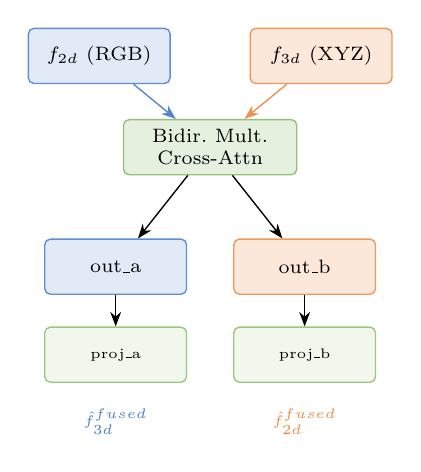
\begin{tikzpicture}[
          every node/.style={font=\scriptsize, align=center},
          fbox/.style={draw, rounded corners=2pt, minimum width=18mm, minimum height=7mm, inner sep=2pt, line width=0.5pt},
          rgb/.style={fbox, fill=RGBStream!15, draw=RGBStream!80},
          xyz/.style={fbox, fill=XYZStream!18, draw=XYZStream!80},
          fuse/.style={fbox, fill=FuseGreen!18, draw=FuseGreen!75, minimum width=22mm},
          arr/.style={->, >=Stealth, line width=0.5pt},
      ]
        \node[rgb] (fr) {$f_{2d}$ (RGB)};
        \node[xyz, right=10mm of fr] (fx) {$f_{3d}$ (XYZ)};
        \node[fuse, below=8mm of $(fr)!0.5!(fx)$] (fuse) {Bidir.~Mult.\\Cross-Attn};
        \node[rgb, below=8mm of fuse, xshift=-12mm] (oa) {out\_a};
        \node[xyz, below=8mm of fuse, xshift=12mm]  (ob) {out\_b};
        \node[fbox, fill=FuseGreen!10, draw=FuseGreen!70, below=4mm of oa, font=\tiny] (pa) {proj\_a};
        \node[fbox, fill=FuseGreen!10, draw=FuseGreen!70, below=4mm of ob, font=\tiny] (pb) {proj\_b};
        \node[font=\tiny, below=2mm of pa, color=RGBStream!90] {$\hat f_{3d}^{\text{fused}}$};
        \node[font=\tiny, below=2mm of pb, color=XYZStream!90] {$\hat f_{2d}^{\text{fused}}$};
        \draw[arr, RGBStream!85] (fr) -- (fuse);
        \draw[arr, XYZStream!85] (fx) -- (fuse);
        \draw[arr] (fuse) -- (oa);
        \draw[arr] (fuse) -- (ob);
        \draw[arr] (oa) -- (pa);
        \draw[arr] (ob) -- (pb);
      \end{tikzpicture}
    \end{column}
  \end{columns}
\end{frame}

% ─── 方法 Frame 3: 多尺度双路网络架构 (TikZ) ───────────
\begin{frame}{多尺度双路网络架构}
  \vspace{-0.4em}
  \begin{center}
  \resizebox{0.98\linewidth}{!}{%
  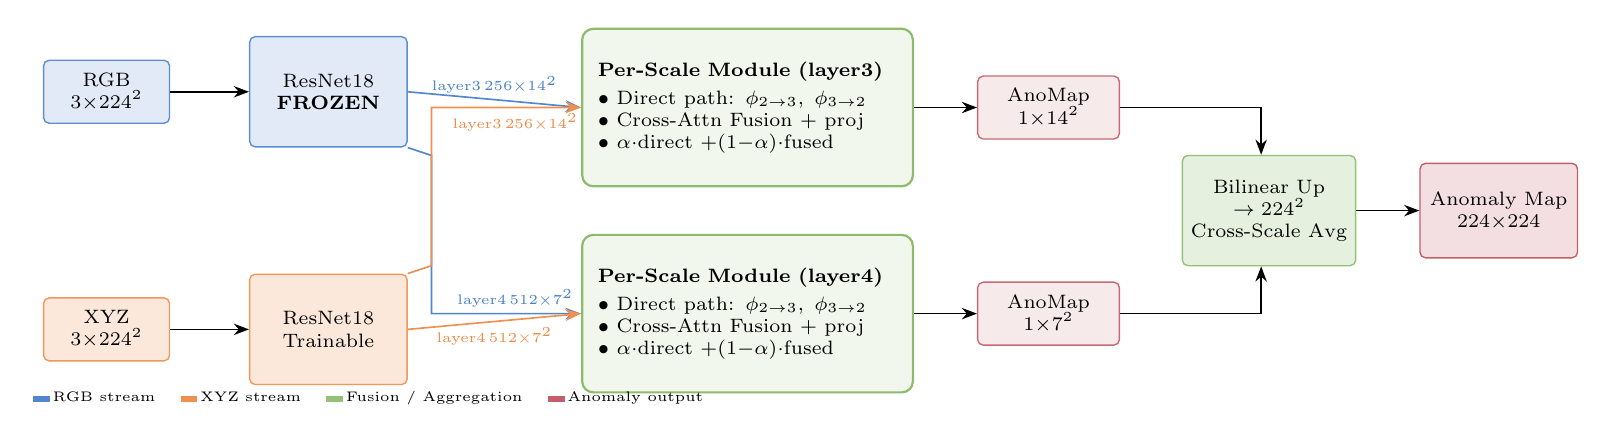
\begin{tikzpicture}[
      every node/.style={font=\scriptsize, align=center},
      box/.style       ={draw, rounded corners=2pt, minimum height=8mm, minimum width=16mm, inner sep=2pt, line width=0.5pt},
      rgb/.style       ={box, fill=RGBStream!15, draw=RGBStream!80},
      xyz/.style       ={box, fill=XYZStream!18, draw=XYZStream!80},
      enc/.style       ={box, minimum width=20mm, minimum height=14mm, font=\scriptsize},
      mod/.style       ={draw=FuseGreen!80, thick, rounded corners=4pt, fill=FuseGreen!10,
                         minimum width=42mm, minimum height=20mm, align=left, inner sep=4pt, text width=38mm},
      outbox/.style    ={box, fill=AccentRed!15, draw=AccentRed!75, minimum width=20mm, minimum height=12mm},
      anomap/.style    ={box, fill=AccentRed!10, draw=AccentRed!70, minimum width=18mm, minimum height=8mm},
      agg/.style       ={box, fill=FuseGreen!18, draw=FuseGreen!75, minimum width=22mm, minimum height=14mm},
      arr/.style       ={->, >=Stealth, line width=0.55pt},
      arrb/.style      ={->, >=Stealth, line width=0.6pt, RGBStream!85},
      arrr/.style      ={->, >=Stealth, line width=0.6pt, XYZStream!85},
      lbl/.style       ={font=\tiny, inner sep=1pt},
  ]
  % ─ Inputs (column 1) ─
  \node[rgb]                                    (rgb) {RGB\\$3{\times}224^2$};
  \node[xyz, below=22mm of rgb]                 (xyz) {XYZ\\$3{\times}224^2$};

  % ─ Encoders (column 2) ─
  \node[rgb, enc, right=10mm of rgb]            (e1)  {ResNet18\\\textbf{FROZEN}};
  \node[xyz, enc, right=10mm of xyz]            (e2)  {ResNet18\\Trainable};

  % ─ Per-Scale Modules (column 3) — l3 top, l4 bottom ─
  \node[mod, right=22mm of e1, yshift=-2mm]
        (mod3) {\textbf{Per-Scale Module (layer3)}\\[2pt]
                \scriptsize $\bullet$ Direct path: $\phi_{2\to3},\;\phi_{3\to2}$\\
                $\bullet$ Cross-Attn Fusion + proj\\
                $\bullet$ $\alpha\cdot$direct $+(1{-}\alpha)\cdot$fused};
  \node[mod, right=22mm of e2, yshift=2mm]
        (mod4) {\textbf{Per-Scale Module (layer4)}\\[2pt]
                \scriptsize $\bullet$ Direct path: $\phi_{2\to3},\;\phi_{3\to2}$\\
                $\bullet$ Cross-Attn Fusion + proj\\
                $\bullet$ $\alpha\cdot$direct $+(1{-}\alpha)\cdot$fused};

  % ─ Per-scale anomaly maps (column 4) ─
  \node[anomap, right=8mm of mod3]              (a3)  {AnoMap\\$1{\times}14^2$};
  \node[anomap, right=8mm of mod4]              (a4)  {AnoMap\\$1{\times}7^2$};

  % ─ Aggregation (column 5) ─
  \node[agg]    at ($(a3)!0.5!(a4) + (28mm,0)$) (aggn) {Bilinear Up\\$\to 224^2$\\Cross-Scale Avg};

  % ─ Final (column 6) ─
  \node[outbox, right=8mm of aggn]              (final) {Anomaly Map\\$224{\times}224$};

  % ─ Arrows: input → encoder ─
  \draw[arr] (rgb) -- (e1);
  \draw[arr] (xyz) -- (e2);

  % ─ Encoder → modules (with scale labels on arrows) ─
  \draw[arrb] (e1.east) -- node[lbl, above=1pt, color=RGBStream!90]
              {\,layer3\,$256{\times}14^2$\,} (mod3.west);
  \draw[arrb] (e1.south east) -- ++(0.3,-0.1) |- node[lbl, pos=0.78, above=1pt, color=RGBStream!90]
              {\,layer4\,$512{\times}7^2$\,} (mod4.west);
  \draw[arrr] (e2.north east) -- ++(0.3,0.1) |- node[lbl, pos=0.78, below=1pt, color=XYZStream!90]
              {\,layer3\,$256{\times}14^2$\,} (mod3.west);
  \draw[arrr] (e2.east) -- node[lbl, below=1pt, color=XYZStream!90]
              {\,layer4\,$512{\times}7^2$\,} (mod4.west);

  % ─ Module → AnoMap ─
  \draw[arr] (mod3) -- (a3);
  \draw[arr] (mod4) -- (a4);

  % ─ AnoMap → Aggregation ─
  \draw[arr] (a3.east) -| ([xshift=-1mm]aggn.north);
  \draw[arr] (a4.east) -| ([xshift=-1mm]aggn.south);

  % ─ Aggregation → Final ─
  \draw[arr] (aggn) -- (final);

  % ─ Legend ─
  \node[font=\tiny, anchor=north west, inner sep=2pt]
        at ([xshift=-2mm,yshift=-3mm]xyz.south west)
        {\textcolor{RGBStream!85}{\rule{6pt}{2pt}}\,RGB stream \quad
         \textcolor{XYZStream!85}{\rule{6pt}{2pt}}\,XYZ stream \quad
         \textcolor{FuseGreen!75}{\rule{6pt}{2pt}}\,Fusion / Aggregation \quad
         \textcolor{AccentRed!75}{\rule{6pt}{2pt}}\,Anomaly output};
  \end{tikzpicture}
  }%
  \end{center}
  \vspace{-0.2em}
  \begin{hlbox}
    \footnotesize
    \textbf{推理时双路加权}：$\text{anomaly} = \alpha\cdot\text{anomaly}_{\text{direct}} + (1-\alpha)\cdot\text{anomaly}_{\text{fused}}$，按尺度独立计算后跨尺度平均得最终热力图。
  \end{hlbox}
\end{frame}

% ════════════════════════════════════════════════════════
\section{实验结果}
% ════════════════════════════════════════════════════════

% ─── 实验 Frame 1: 训练曲线 (cookie 三 seed) ───────────
\begin{frame}{Cookie 类别 · 三随机种子可复现性}
  \vspace{-0.4em}
  \begin{center}
  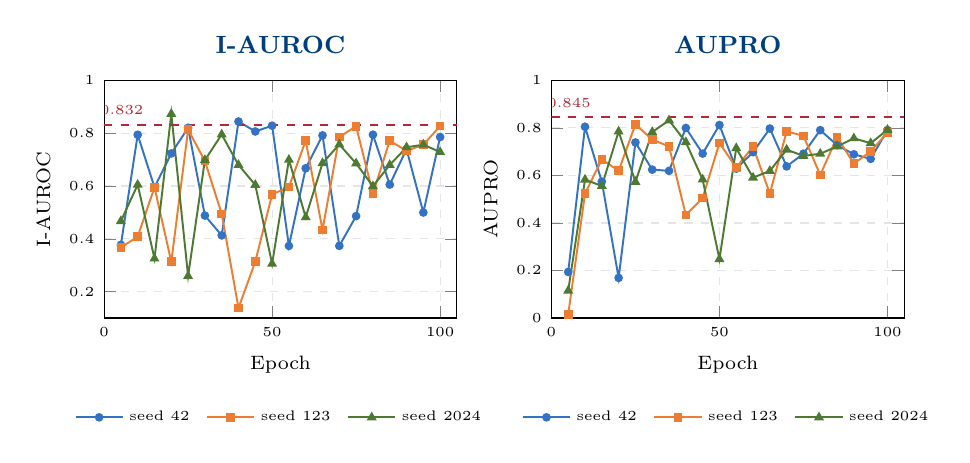
\begin{tikzpicture}
  \begin{axis}[
      name=plotA,
      width=0.50\linewidth, height=4.6cm,
      title={\small I-AUROC},
      xlabel={\scriptsize Epoch}, ylabel={\scriptsize I-AUROC},
      ymin=0.1, ymax=1.0,
      xmin=0, xmax=105,
      grid=both, grid style={gray!20, dashed},
      legend style={font=\tiny, at={(0.5,-0.34)}, anchor=north, /tikz/every even column/.append style={column sep=4pt}, draw=none, fill=none, legend columns=3},
      tick label style={font=\tiny},
      title style={font=\small\bfseries, color=ZJUBlue},
      label style={font=\scriptsize},
  ]
  \addplot[color=RGBStream, mark=*, mark size=1.2pt, line width=0.7pt] coordinates {
    (5,0.3773)(10,0.7940)(15,0.5950)(20,0.7233)(25,0.8204)(30,0.4879)(35,0.4130)(40,0.8443)(45,0.8065)(50,0.8284)(55,0.3731)(60,0.6671)(65,0.7916)(70,0.3734)(75,0.4861)(80,0.7944)(85,0.6054)(90,0.7393)(95,0.4997)(100,0.7854)
  }; \addlegendentry{seed 42}
  \addplot[color=XYZStream, mark=square*, mark size=1.2pt, line width=0.7pt] coordinates {
    (5,0.3672)(10,0.4081)(15,0.5950)(20,0.3131)(25,0.8135)(30,0.6945)(35,0.4945)(40,0.1380)(45,0.3135)(50,0.5683)(55,0.5964)(60,0.7718)(65,0.4334)(70,0.7857)(75,0.8263)(80,0.5714)(85,0.7715)(90,0.7330)(95,0.7562)(100,0.8273)
  }; \addlegendentry{seed 123}
  \addplot[color=FuseGreen!70!black, mark=triangle*, mark size=1.4pt, line width=0.7pt] coordinates {
    (5,0.4671)(10,0.6047)(15,0.3252)(20,0.8731)(25,0.2590)(30,0.6980)(35,0.7951)(40,0.6796)(45,0.6040)(50,0.3055)(55,0.6994)(60,0.4816)(65,0.6865)(70,0.7573)(75,0.6855)(80,0.5992)(85,0.6796)(90,0.7465)(95,0.7566)(100,0.7285)
  }; \addlegendentry{seed 2024}
  \draw[AccentRed, dashed, line width=0.6pt] (axis cs:0,0.832) -- (axis cs:105,0.832) node[pos=0.05, above, font=\tiny, color=AccentRed]{0.832};
  \end{axis}

  \begin{axis}[
      at={(plotA.east)}, anchor=west, xshift=12mm,
      width=0.50\linewidth, height=4.6cm,
      title={\small AUPRO},
      xlabel={\scriptsize Epoch}, ylabel={\scriptsize AUPRO},
      ymin=0, ymax=1.0,
      xmin=0, xmax=105,
      grid=both, grid style={gray!20, dashed},
      legend style={font=\tiny, at={(0.5,-0.34)}, anchor=north, /tikz/every even column/.append style={column sep=4pt}, draw=none, fill=none, legend columns=3},
      tick label style={font=\tiny},
      title style={font=\small\bfseries, color=ZJUBlue},
      label style={font=\scriptsize},
  ]
  \addplot[color=RGBStream, mark=*, mark size=1.2pt, line width=0.7pt] coordinates {
    (5,0.1940)(10,0.8048)(15,0.5738)(20,0.1689)(25,0.7387)(30,0.6245)(35,0.6192)(40,0.7997)(45,0.6918)(50,0.8121)(55,0.6284)(60,0.6978)(65,0.7972)(70,0.6381)(75,0.6916)(80,0.7905)(85,0.7275)(90,0.6889)(95,0.6699)(100,0.7908)
  }; \addlegendentry{seed 42}
  \addplot[color=XYZStream, mark=square*, mark size=1.2pt, line width=0.7pt] coordinates {
    (5,0.0158)(10,0.5236)(15,0.6677)(20,0.6196)(25,0.8148)(30,0.7511)(35,0.7221)(40,0.4336)(45,0.5053)(50,0.7366)(55,0.6330)(60,0.7213)(65,0.5238)(70,0.7854)(75,0.7664)(80,0.6018)(85,0.7617)(90,0.6494)(95,0.7014)(100,0.7806)
  }; \addlegendentry{seed 123}
  \addplot[color=FuseGreen!70!black, mark=triangle*, mark size=1.4pt, line width=0.7pt] coordinates {
    (5,0.1154)(10,0.5825)(15,0.5557)(20,0.7848)(25,0.5729)(30,0.7825)(35,0.8317)(40,0.7400)(45,0.5829)(50,0.2480)(55,0.7148)(60,0.5906)(65,0.6191)(70,0.7086)(75,0.6820)(80,0.6914)(85,0.7218)(90,0.7561)(95,0.7358)(100,0.7918)
  }; \addlegendentry{seed 2024}
  \draw[AccentRed, dashed, line width=0.6pt] (axis cs:0,0.845) -- (axis cs:105,0.845) node[pos=0.05, above, font=\tiny, color=AccentRed]{0.845};
  \end{axis}
  \end{tikzpicture}
  \end{center}
  \vspace{-0.4em}
  \begin{hlbox}
    \footnotesize
    三 seed 峰值均突破 \textbf{I-AUROC = 0.83 / AUPRO = 0.81}，最优峰值 \textbf{I-AUROC = 0.832, AUPRO = 0.845}；峰值 std $<$ 0.01，方法可复现性良好。
  \end{hlbox}
\end{frame}

% ─── 实验 Frame 2: Cookie 对原论文 baseline ───────────
\begin{frame}{Cookie 类 · 对比原论文最优 baseline}
  \vspace{-0.3em}
  \begin{columns}[T]
    \begin{column}{0.42\textwidth}
      \vspace{0.4em}
      \begin{block}{Cookie 指标对比}
        \scriptsize
        \centering
        \renewcommand{\arraystretch}{1.30}
        \setlength{\tabcolsep}{4pt}
        \begin{tabular}{lcc}
          \textbf{Method} & \textbf{I-AUROC} & \textbf{AUPRO} \\
          \midrule
          原论文最优 & 0.701 & 0.740 \\
          \textbf{本方法} & \textcolor{AccentRed}{\textbf{0.832}} & \textcolor{AccentRed}{\textbf{0.845}} \\
          \midrule
          $\Delta$ & \textcolor{AccentRed}{\textbf{+0.131}} & \textcolor{AccentRed}{\textbf{+0.105}} \\
        \end{tabular}
      \end{block}
      \vspace{0.6em}
      \begin{itemize}\footnotesize
        \item[\cmark] I-AUROC、AUPRO 双指标\textbf{超越 baseline}
        \item[\cmark] 验证多尺度跨注意力融合的有效性
      \end{itemize}
    \end{column}
    \begin{column}{0.58\textwidth}
      \centering
      \footnotesize\color{AccentGray}原论文 I-AUROC 表 · cookie 最优 0.701\\[0.2em]
      \includegraphics[width=\linewidth]{images/2026-05-03-21-04-11.png}\\[0.4em]
      \footnotesize\color{AccentGray}原论文 AUPRO 表 · cookie 最优 0.740\\[0.2em]
      \includegraphics[width=\linewidth]{images/2026-05-03-21-01-47.png}
    \end{column}
  \end{columns}
\end{frame}

% ─── 实验 Frame 3: 跨类别泛化 ──────────────────────────
\begin{frame}{跨类别泛化}
  \vspace{-0.2em}
  \begin{columns}[T]
    \begin{column}{0.45\textwidth}
      \begin{block}{三类别峰值}
        \footnotesize
        \centering
        \renewcommand{\arraystretch}{1.25}
        \begin{tabular}{lcc}
          \toprule
          \textbf{Category} & \textbf{I-AUROC} & \textbf{AUPRO} \\
          \midrule
          \rowcolor{ZJULight}
          \textbf{cookie} & \textbf{0.832} & \textbf{0.845} \\
          dowel           & 0.870 & 0.730 \\
          cable\_gland    & 0.591 & 0.707 \\
          \bottomrule
        \end{tabular}
      \end{block}
      \vspace{0.6em}
      \begin{hlbox}
        \centering\footnotesize
        具备一定的\textbf{跨类别泛化能力}。
      \end{hlbox}
    \end{column}
    \begin{column}{0.55\textwidth}
      \begin{hlbox}[title=猜测问题：冻结策略不通用]
        \footnotesize
        RGB 编码器冻结对 cookie 类影响较小，但某些工业表面特征更复杂、难以适用；后续将引入\textbf{动态冻结机制}，针对不同类别调整冻结策略。
      \end{hlbox}
    \end{column}
  \end{columns}
\end{frame}

% ════════════════════════════════════════════════════════
\section{总结与展望}
% ════════════════════════════════════════════════════════

\begin{frame}{总结与未来工作}
  \vspace{-0.2em}
  \begin{columns}[T]
    \begin{column}{0.50\textwidth}
      \begin{block}{已取得成果}
        \footnotesize
        \begin{itemize}\footnotesize
          \item[\cmark] \textbf{检测性能}：cookie 类 I-AUROC = 0.832 / AUPRO = 0.845，相比原论文最优 baseline 分别提升 \textbf{+0.131 / +0.105}
          \item[\cmark] \textbf{可复现性}：三 seed 峰值 std $<$ 0.01
          \item[\cmark] \textbf{泛化能力}：直接迁移至 dowel、cable\_gland 类别同样取得有效结果，体现架构的一定鲁棒性
          \item[\cmark] \textbf{方法贡献}：跨模态映射 + 多尺度双向乘性跨注意力融合的 normal-only 框架
        \end{itemize}
      \end{block}
    \end{column}
    \begin{column}{0.50\textwidth}
      \begin{block}{后续研究方向（局限与优化）}
        \footnotesize
        \begin{itemize}\footnotesize
          \item[\xmark] \textbf{训练指标震荡}：训练过程指标存在明显震荡，计划引入\textbf{学习率预热}配合\textbf{更平滑的退火策略}
          \item[\xmark] \textbf{冻结策略不通用}：RGB 编码器冻结对 cookie 类影响较小，但某些工业表面特征更复杂、难以适用；后续将引入\textbf{动态冻结机制}，针对不同类别调整冻结策略
        \end{itemize}
      \end{block}
    \end{column}
  \end{columns}
  \vspace{0.4em}
  \begin{hlbox}
    \centering\footnotesize
    \textbf{核心贡献}：以"跨模态特征映射 + 多尺度双向乘性跨注意力融合"为骨架的 normal-only 工业异常检测框架，已在 cookie 主类别完成系统性验证并超越原论文 baseline，下一阶段聚焦训练稳定性与冻结策略的自适应化。
  \end{hlbox}
\end{frame}

% ─── 谢谢 ──────────────────────────────────────────────
\begin{frame}[plain]
  \vfill
  \begin{center}
    \begin{tikzpicture}
      \node[fill=ZJUBlue,text=white,minimum width=0.7\paperwidth,
            minimum height=3.5cm,inner sep=10pt,align=center] {
        {\Huge\bfseries 谢\,\,谢\,\,聆\,\,听}\\[0.5em]
        {\Large 敬请批评指正}
      };
    \end{tikzpicture}
  \end{center}
  \vfill
  \begin{center}
    \small\color{AccentGray}
    王昱人\quad|\quad \texttt{Albert112358@outlook.com}\quad|\quad 浙江大学 控制科学与工程学院
  \end{center}
  \vfill
\end{frame}

\end{document}